\documentclass[12pt]{article}
\usepackage[latin1]{inputenc}
\usepackage{graphicx,subfigure}
\usepackage{float}
\topmargin -1mm
\oddsidemargin -1mm
\evensidemargin -1mm
\textwidth 165mm
\textheight 220mm
\parskip 2mm
\parindent 3mm
%\pagestyle{empty}

\begin{document}



\begin{center}


{\Large \bf Virtual Calphad Laboratory}


An open-source software for CALPHAD Calculations



\bigskip

\begin{figure}[H]
\centering

\includegraphics[width=20mm]{figs/bagua.png}
\end{figure}

\bigskip
written by Xing Wang

\bigskip

Central South University, China

\bigskip

Version 0.1

\bigskip

{\Large \bf }

\end{center}


\bigskip

\newpage


\newpage

\tableofcontents

\newpage

\section{Preface}

~~I start to wrote VCLab in September. Two month passed, VCLab-0.1 was born, with about 6000 lines code. I don't know if I will continue my work in the field of CALPHAD. So I guess it is time to write a documentation and end this stage of work.


Apart from software, one other thing I wish to do is establish a platform for open source database. Everyone could submit their own database to this platform, and everyone can edit, improve and use it, like Wikipedia. This is a big project need great efforts of CALPHAD community.

Today is my father's 50th birthday, To father's love.
\\
\\
\begin{flushright}
Xing Wang

November 14, 2015
\end{flushright}


\section{Introduction}

VCLab (Virtual Calphad Laboratory) is a open source software for CALPHAD calculations, written in C++.




\section{Installation}

To be added.


\section{Input files}
The VCLInput.txt is the central input file of VCLab. It determines what to do and how to do it.
One example for this file list below:

\begin{table}[!hbp]
\begin{tabular}{l l l }%��ʼ���Ʊ���
Mode                  & = & Equilibrium \\
Dimension             & = & 1 !\\
Database File         & = & AlZn.TDB! \\
Elements		      & = & Al, Zn!\\
Compositions	      & = & 0.6, 0.4!\\
Pressure	          & = & 101325!\\
Variables		      & = & Temperature !\\
V Start		          & = & 300 !\\
V End		          & = & 2000 !\\
V Interval	          & = & 10 !\\
Result Output File	  & = & Result.txt !\\
Global Grid Interval  & = & 0.05 !\\
\end{tabular}
\end{table}

Each line consists of a keyword (i.e. a string) the equation sign "=" and one or several values. Values are separated by a colon ",". One parameter one single line ended by !. Comments are normally preceded by the number sign \#. Defaults are supplied for some parameters. For example, a default for the "Global Grid Interval" is 0.5.

The following sections will describe the parameters given in the VCLInput file.

\subsection{Dimension}
This tag determines the number of variables. $n$D means n variables. $0$D corresponding single point calculation in Thermo-Calc, $1$D is step, $2$D is map. VCLab can handel
any number of variables.


\subsection{Mode}
This flag determines what property to calculate.

(1) Equilibrium

Calculate the thermodynamic equilibrium

(2) Gibbs energy surface

Calculate the Gibbs energy surface of specific phase.


Properties not implemented yet:

(1) Elastic

Calculate the single crystal elastic constants and poly-crystal elastic modules of specific phase.

To be added.


\subsection{Database File}
Database has the same format used in commercial software like Thermo-Calc and Pandat. One could put the Database file in the same folder with VCLab, or give the relative path of it, for instance ..$\backslash$ TDB $\backslash$ AlZn.TDB

\subsection{Variables}
Number of variables must equal to dimension value. The start, end and interval values also should be given.

\subsection{Global Grid Interval}
This flag determines mesh size for creating the global grid point.

\section{Gibbs energy surface}

\subsection{1D}
Example file of VCLInput:

\noindent
Mode~~~~~~~~~~~~~~~~~~~~~~~= ~~ Energy Surface ~~!\\
Database\_File~~~~~~~~~~~~= ~~ AlZn.TDB~~~~~~~~! \\
Elements~~~~~~~~~~~~~~~~~~= ~~ Al, Zn~~~~~~~~~~!\\
Phases\_Selected~~~~~~~~~~= ~~ Liquid, HCP\_A3, FCC\_A1 ~~! \\
Phases\_Rejected~~~~~~~~~= ~~ none ~~! \\
Pressure~~~~~~~~~~~~~~~~~~~= ~~ 101325~~!\\
Temperature~~~~~~~~~~~~~= ~~ 550 ~~!\\
Global\_Grid\_Interval~~~= ~~ 0.02 ~~!\\

Running times: 0.009 s.


\begin{figure}
\subfigure[]{
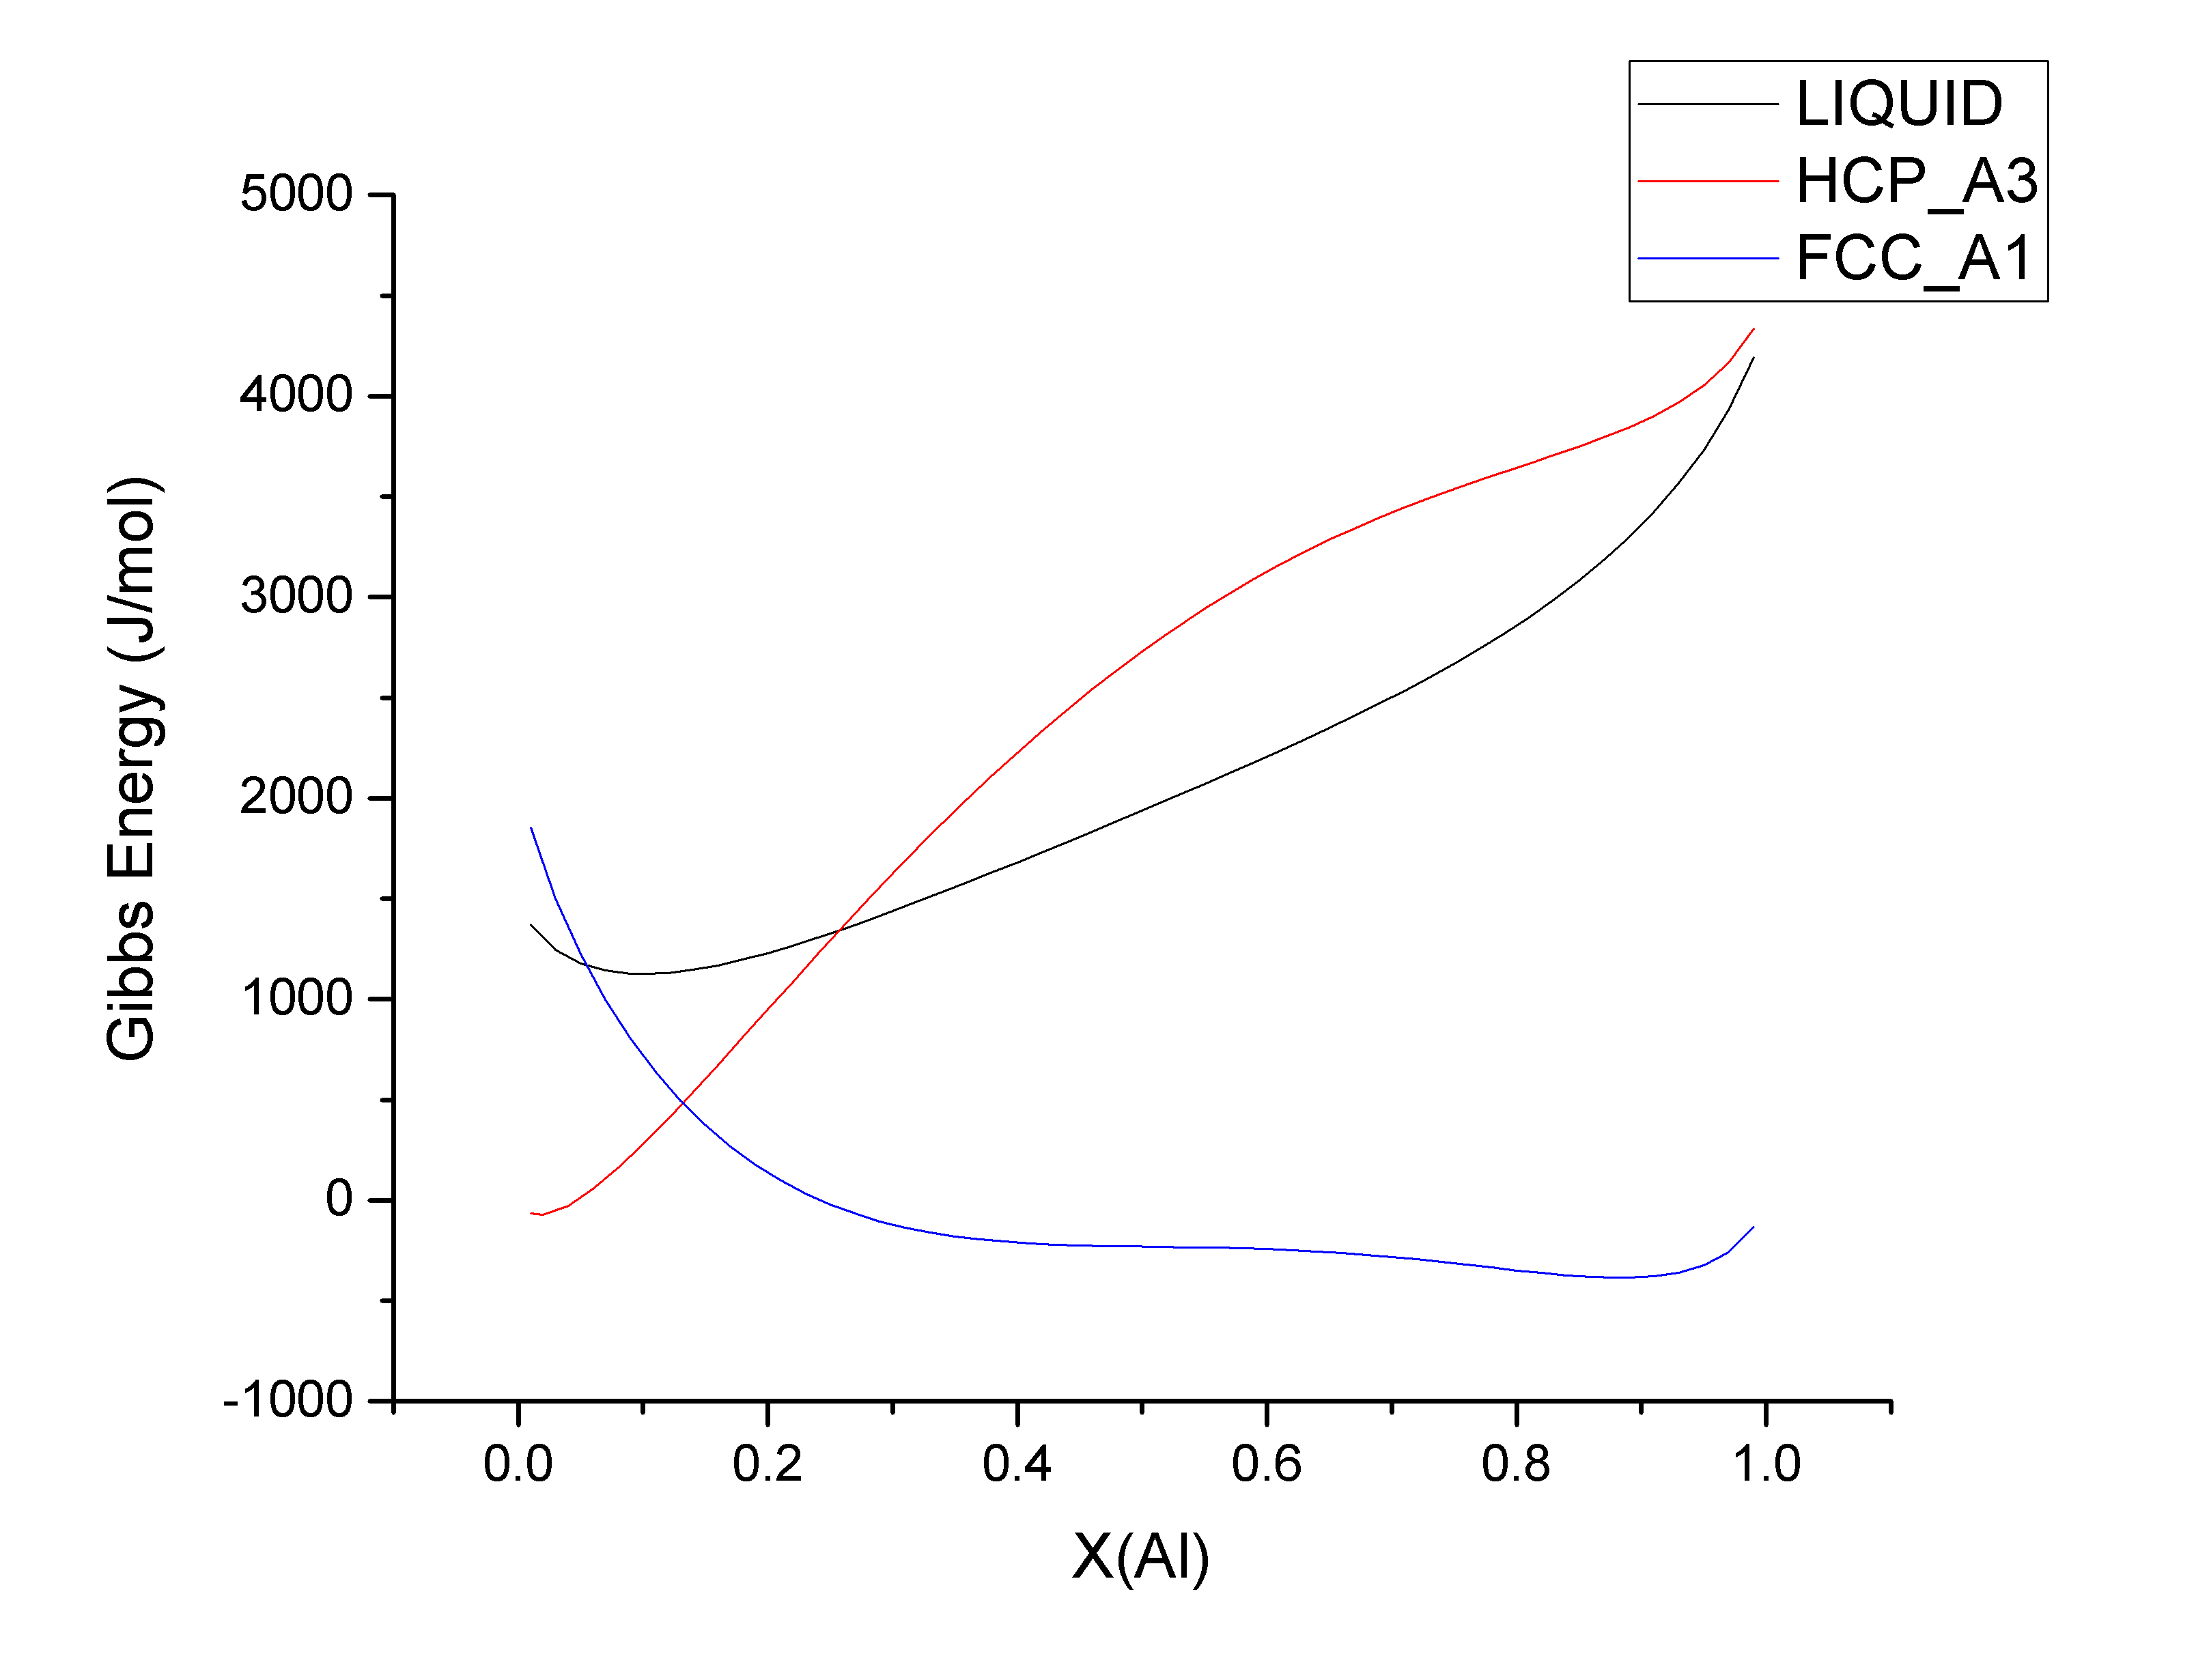
\includegraphics[width=80mm]{figs/ALZN.jpg}}
\subfigure[]{
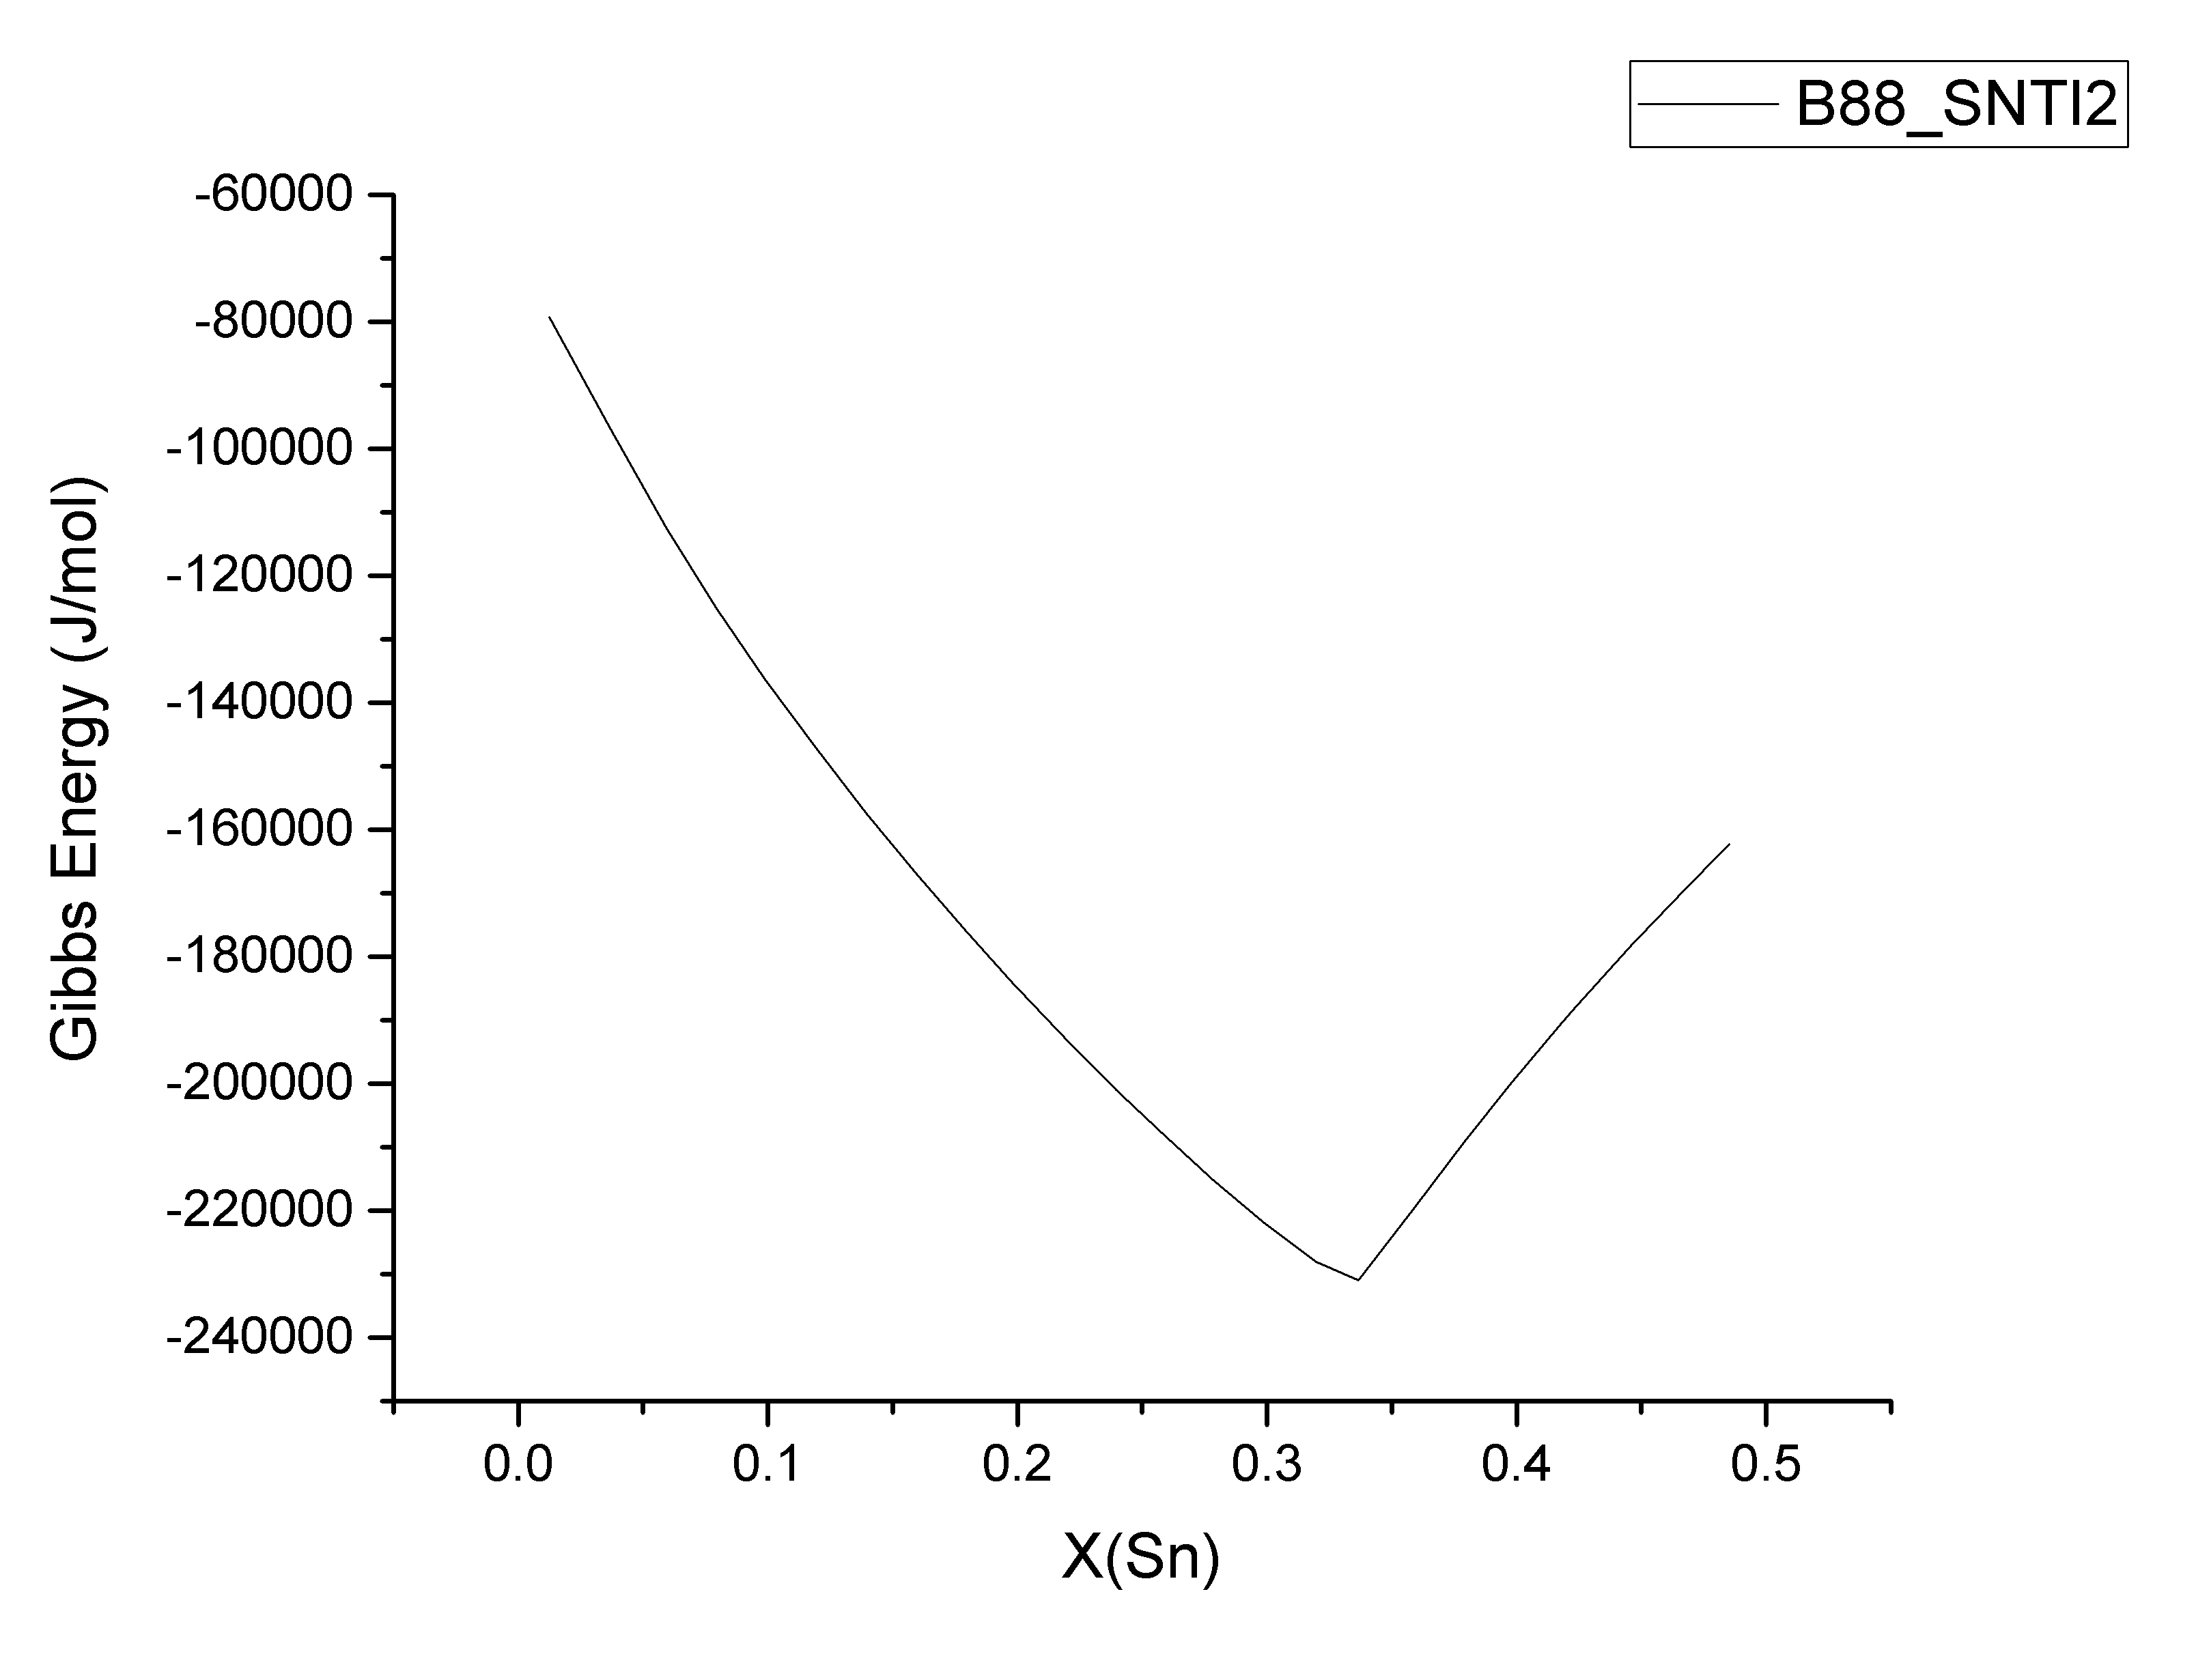
\includegraphics[width=80mm]{figs/B88_SNTI2.jpg}}
\caption{The Gibbs energy curves. (a) Al-Zn binary with one sublattices;
(b) B88\_STi2 phase with two sublattices.}\label{fg:femogrid}
\end{figure}


\subsection{2D}
Example file of VCLInput:

\noindent
Mode~~~~~~~~~~~~~~~~~~~~~~~= ~~ Energy Surface ~~!\\
Database\_File~~~~~~~~~~~~= ~~ cusnti.TDB ~~! \\
Elements~~~~~~~~~~~~~~~~~~= ~~ cu, sn, ti ~~!\\
Phases\_Selected~~~~~~~~~~= ~~ BCC\_A2 ~~! \\
Phases\_Rejected~~~~~~~~~= ~~ none  ~~! \\
Pressure~~~~~~~~~~~~~~~~~~~= ~~ 101325 ~~!\\
Temperature~~~~~~~~~~~~~= ~~ 800 ~~!\\
Global\_Grid\_Interval~~~= ~~ 0.02 ~~!\\

Running times: 0.137 s.

\begin{figure}

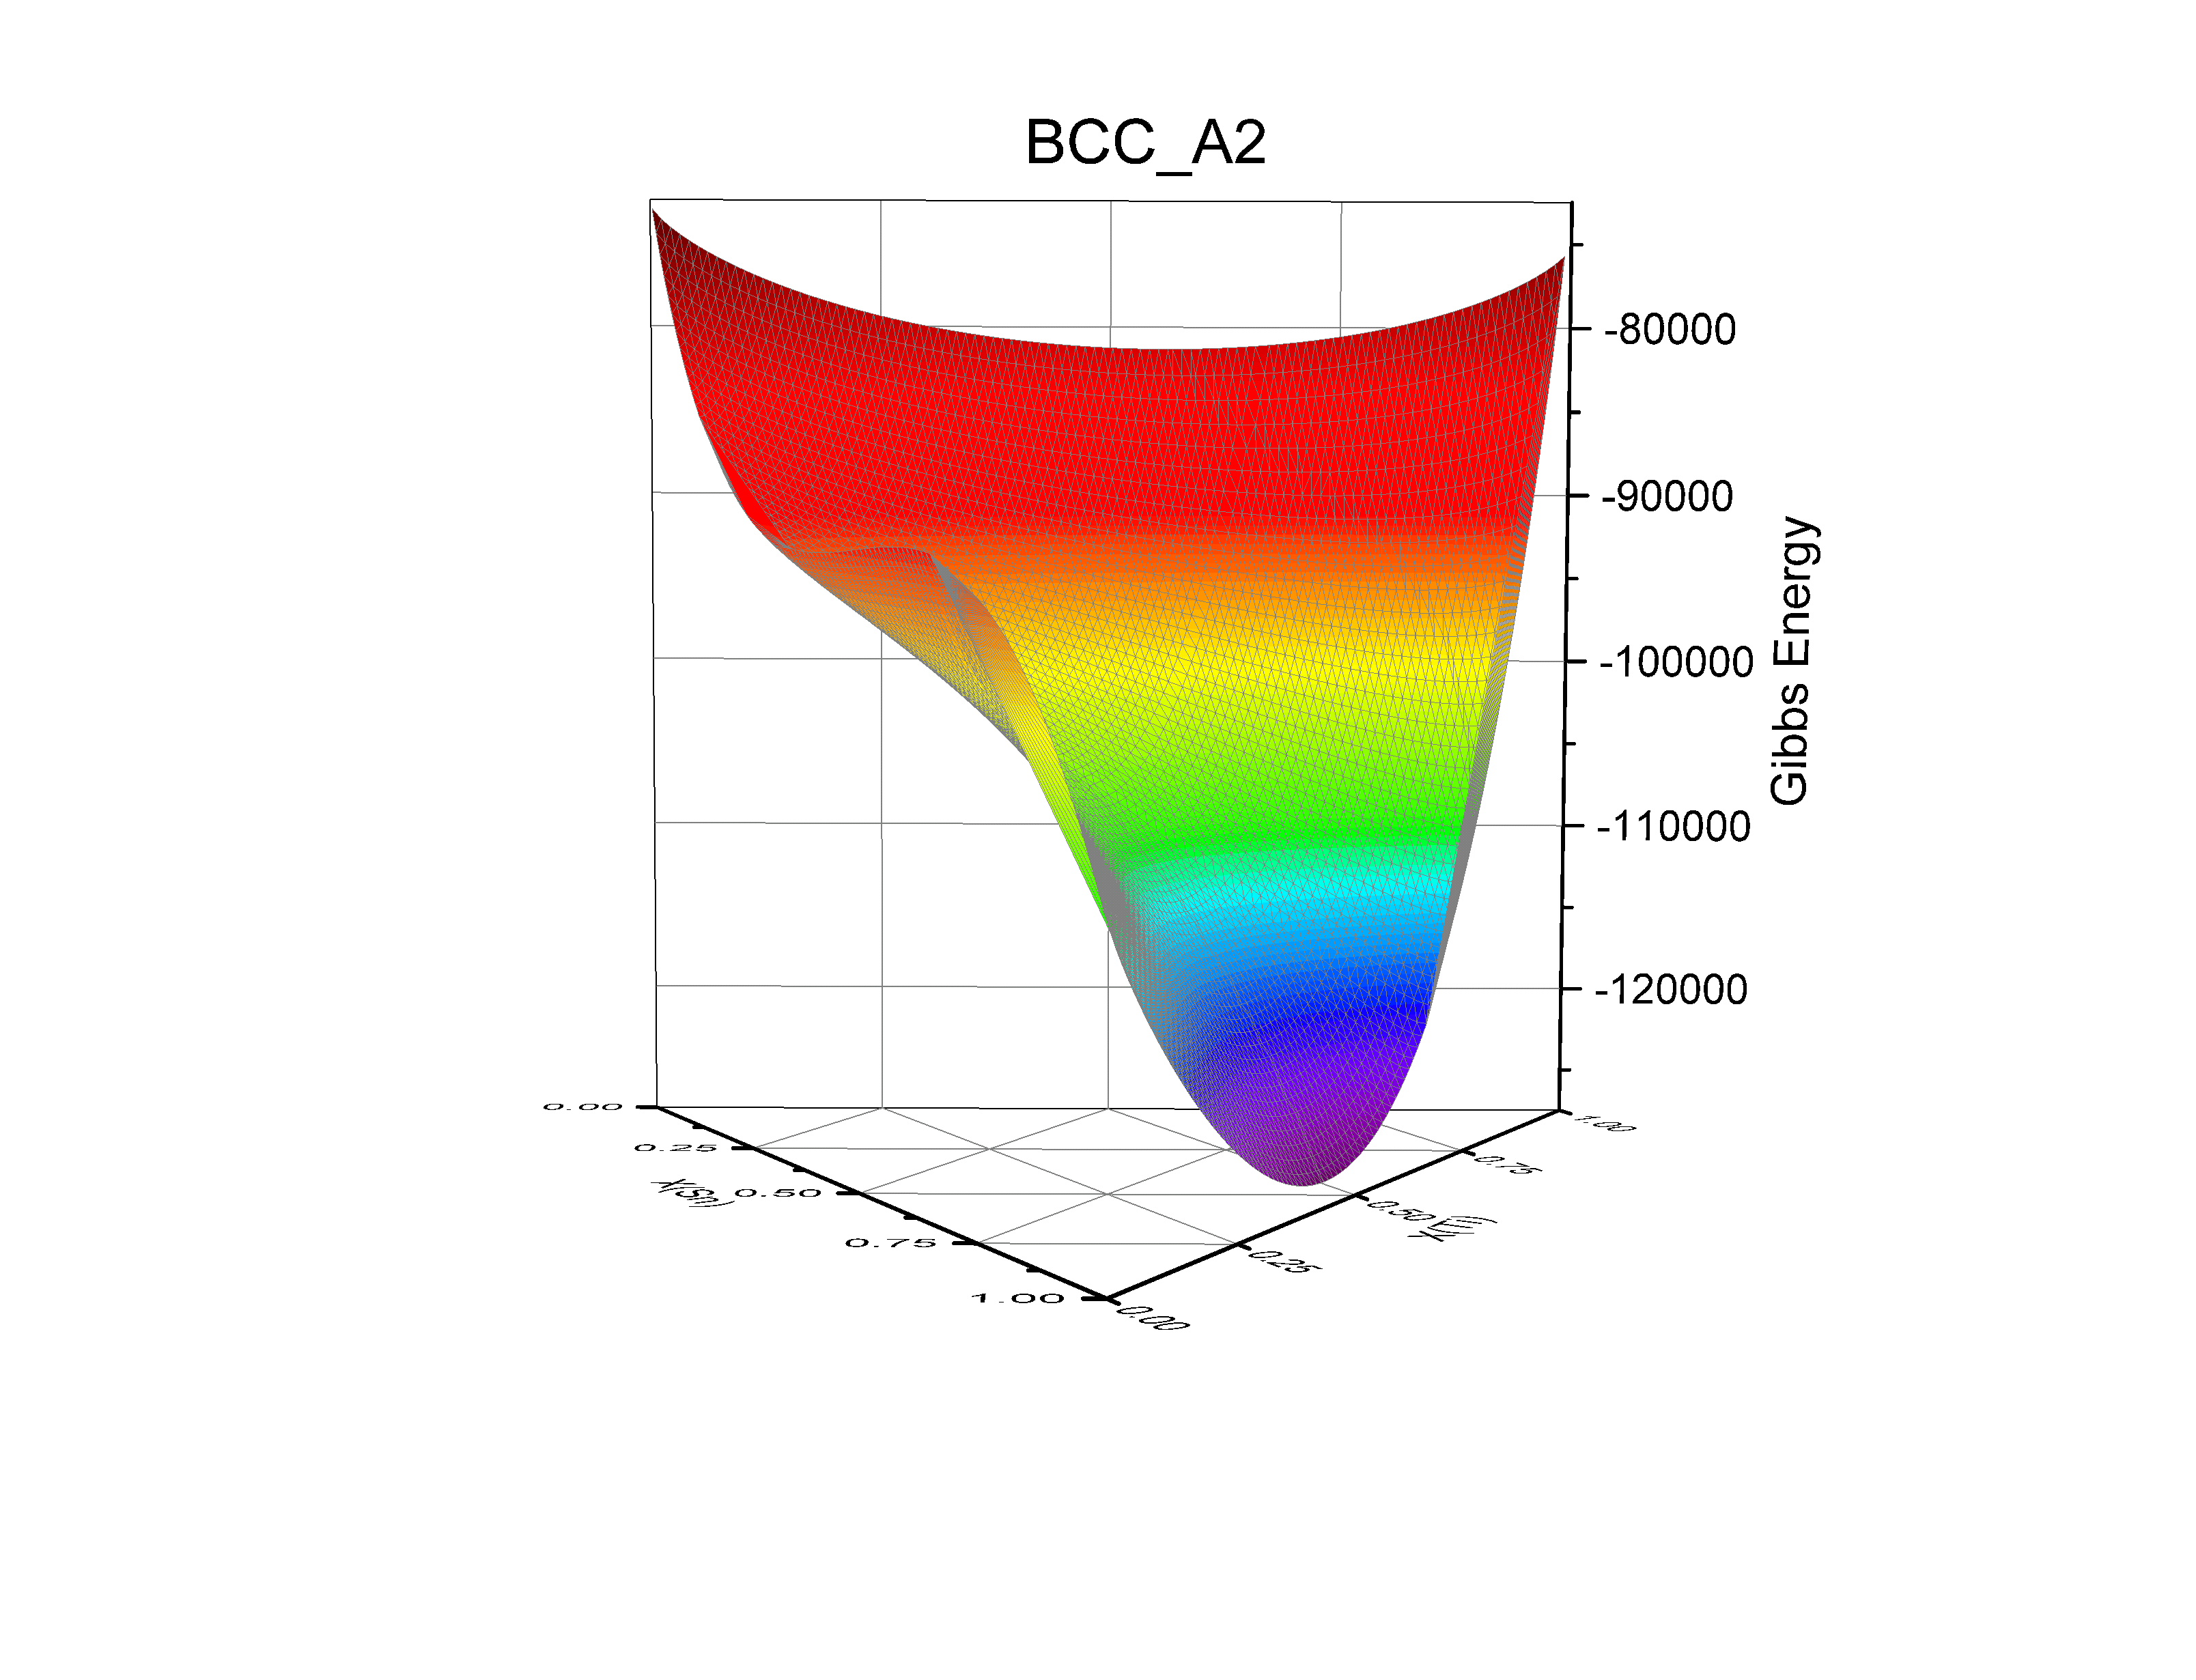
\includegraphics[width=120mm]{figs/BCC_A2.png}

\caption{The Gibbs energy surface of BCC\_A2 Phases in Cu-Sn-Ti ternary system.}\label{fg:femogrid}
\end{figure}


\section{Equilibrium Calculations}

\subsection{Single point}
\subsubsection{Fixed x and T}
Example file of VCLInput:

\noindent
Mode~~~~~~~~~~~~~~~~~~~~~~~= ~~ Equilibrium ~~!\\
Dimension~~~~~~~~~~~~~~~~~= ~~ 0 ~~!\\
Database\_File~~~~~~~~~~~~= ~~ AlZn.TDB ~~! \\
Elements~~~~~~~~~~~~~~~~~~= ~~ Al, Zn ~~!\\
Phases\_Selected~~~~~~~~~~= ~~ all ~~! \\
Phases\_Rejected~~~~~~~~~= ~~ none  ~~! \\
Pressure~~~~~~~~~~~~~~~~~~~= ~~ 101325 ~~!\\
Temperature~~~~~~~~~~~~~= ~~ 600 ~~!\\
Compositions~~~~~~~~~~~~= ~~ 0.6, 0.4 ~~!\\
Global\_Grid\_Interval~~~= ~~ 0.02 ~~!\\

Equilibrium can be found in the VCLOutput.txt file. A example is list below:

\noindent
====================================================\\
Conditions:   T = 600   P = 10500   N = 1\\
   X(AL) = 0.7\\
   X(ZN) = 0.3\\
====================================================\\

Equilibrium:

Chemical potential:\\
AL   580.969\\
ZN   495.04\\

Phase:\\
FCC\_A1\#2\\
Moles: 0.702168\\
X(AL) = 0.777535\\
X(ZN) = 0.222465\\

FCC\_A1\\
Moles: 0.297832\\
X(AL) = 0.517203\\
X(ZN) = 0.482797\\

Running times: 0.027 s.

\subsubsection{Fixed x and Phase}

To be added.


\subsection{Step}
Example file of VCLInput:
\noindent
Mode~~~~~~~~~~~~~~~~~~~~~~~= ~~ Equilibrium ~~!\\
Dimension~~~~~~~~~~~~~~~~~= ~~ 1 ~~!\\
Database\_File~~~~~~~~~~~~= ~~ cusnti.TDB ~~! \\
Elements~~~~~~~~~~~~~~~~~~= ~~ cu, sn, ti ~~!\\
Compositions~~~~~~~~~~~~= ~~ 0.1, 0.6, 0.3 ~~!\\
Phases\_Selected~~~~~~~~~~= ~~ all ~~! \\
Phases\_Rejected~~~~~~~~~= ~~ none  ~~! \\
Pressure~~~~~~~~~~~~~~~~~~~= ~~ 101325 ~~!\\
Variables~~~~~~~~~~~~~~~~~~= ~~ Temperature ~~!\\
V\_start~~~~~~~~~~~~~~~~~~~~= ~~ 300 ~~!\\
V\_end~~~~~~~~~~~~~~~~~~~~~= ~~ 2000 ~~!\\
V\_Interval~~~~~~~~~~~~~~~~= ~~ 5 ~~!\\
Global\_Grid\_Interval~~~= ~~ 0.02 ~~!\\

Running times: 2.137 s.

Results of phase fractions are stored in phase farctions.txt file. One examples in Cu-Sn-Ti ternary system is show in Fig.~\ref{fg:cusnti} 

\begin{figure}
\subfigure[]{
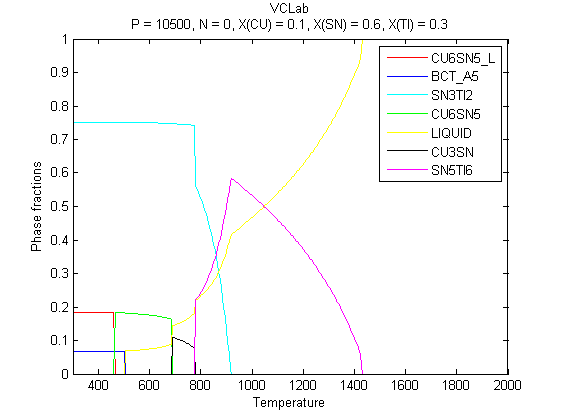
\includegraphics[width=80mm]{figs/CuSnTi.png}}
\subfigure[]{
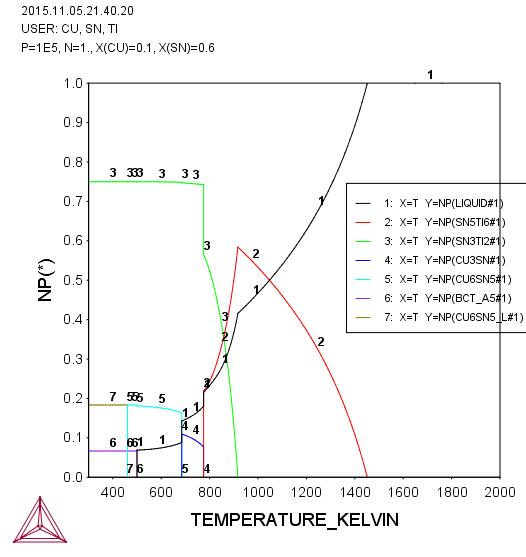
\includegraphics[width=80mm]{figs/TC_CuSnTi.jpg}}
\caption{ Equilibrium solidification process of a Cu-Sn-Ti alloys. (a) VCLab;
(b) Thermo-Calc 2015 demo version.}\label{fg:cusnti}
\end{figure}


\subsection{Map}
To be added.

\subsection{High dimensions calculations}
To be added.

\section{Algorithm}

The algorithm to calculate thermodynamic equilibria for
multi-component systems was widely introduced in varies papers
and books. In this document, the algorithm is explained in the
way that directly relate to programming.
\subsection{Gibbs energy function}
In thermodynamics, phases equilibrium is a state when the chemical potential
in all phases are equal for every component at given conditions. In mathematics, phases
equilibrium is the global minimum point of the overall Gibbs energy function,
with given constraints.

The Gibbs energy function can be written as:
\begin{equation}
G = \sum_{\alpha} n^{\alpha} G^{\alpha}(T,P,y^{\alpha}_{ks}) \label{eq:gsum}
\end{equation}
where $n^{\alpha}$ is the moles amount of the phase $\alpha$ and
$G^{\alpha}$ is the Gibbs energy per mole formula of phase $\alpha$. T and P
is the temperature and pressure, $y^{\alpha}_{ks}$ is the site fractions in the
 s lattices of phase $\alpha$.

\noindent
The equality constraint are:

(1) sum of the site fractions on sublattice s of phase $\alpha$ should be unity:
\begin{equation}
\sum_k y^{\alpha}_{ks} - 1= 0
\end{equation}

(2) sum of the components amount should equal to overall components amount:
\begin{equation}
\sum_{\alpha}n^{\alpha}N^{\alpha}_{A} - \tilde N_{A}=0
\end{equation}

\noindent
where ${\tilde N}_{A}$ is the overall amount of component A.



The inequality constraint are:
\begin{equation}
\ y^{\alpha}_{ks} > 0
\end{equation}

\begin{equation}
\ n^{\alpha} > 0
\end{equation}

\noindent
charge balance is not consider at the moment.


\subsection{Lagrangian method}
A strategy for finding the minima of a function subject to equality
constraints is lagrangian methods. Lagrange multipliers can be used
to convert it into an unconstrained problem whose number of variables
is the original number of variables plus the original number of
equality constraints.

\begin{equation}
L = G + \sum_{\alpha} \lambda_s^{\alpha} (\sum_k y^{s, \alpha}_{k} - 1)
+ \sum_{A} \mu_{A}(\sum_{\alpha}n^{\alpha}N^{\alpha}_{A} - \tilde N_{A})
\end{equation}
\noindent
where $\lambda^{\alpha}, \mu_{\rm A}$ are multipliers.

The minimum can be reach, when the derivative of the Lagrangian with
respect to all the variables are zeros.

\begin{equation}
G^{\alpha}_M + \sum_{A} \mu_{A} N^{\alpha}_{A} = 0
\end{equation}

\begin{equation}
\sum_k y^{s, \alpha}_{k} - 1= 0
\end{equation}

\begin{equation}
n^{\alpha}\frac{\partial G^{\alpha}}{\partial y^{s, \alpha}_{k}}
- n^{\alpha}\mu_{A}\frac{\partial N^{\alpha}_{A}}{\partial y^{s, \alpha}_{k}}
- \lambda_s^{\alpha} = 0
\end{equation}

\begin{equation}
\sum_{\alpha}n^{\alpha}N^{\alpha}_{A} - \tilde N_{A}=0
\end{equation}

In order to solve this nonlinear equations, Newton's method can be used.
We then get:


\refstepcounter{equation}\label{eq:HillertMatrix}

\[
\left(
\begin{tabular}{cccccc}
 0 & 1 & 0 & 0 & 0 &0\\
\\
1 & $\frac{\partial^2 G^{\alpha}}{\partial y_k^{s, \alpha}\partial y_{k^{\prime}}^{s, \alpha}} $ &
0 & $\frac{\partial N^{\alpha}_{A}}{\partial y^{s, \alpha}_{k}}$
& $\frac{\partial^2 G^{\alpha}}{\partial y_k^{s, \alpha} \partial T}$
& $\frac{\partial^2 G^{\alpha}}{\partial y_k^{s, \alpha} \partial P}$ \\
\\
0 & $\frac{\partial G^{\alpha}}{\partial y_k^{s, \alpha}} +
\mu_{A}\frac{\partial N^{\alpha}_{A}}{\partial y^{s, \alpha}_{k}}$
& 0 & $N^{\alpha}_{A}$
& $\frac{\partial G^{\alpha}}{\partial T}$
& $\frac{\partial G^{\alpha}}{\partial T}$  \\
\\
 0 & $n^{\alpha}\frac{\partial N^{\alpha}_{A}}{\partial y^{s, \alpha}_{k}}$
 & $N^{\alpha}_{A}$ & 0 & 0 & 0\\
\end{tabular}
\right)
\left(
\begin{tabular}{c}

$\Delta \lambda_s^{\alpha}$\\
\\
$\Delta y^{s, \alpha}_{k}$\\
\\
$\Delta n^{\alpha}$\\
\\
$\Delta \mu_{A}$\\
\\
$\Delta T$\\
\\
$\Delta P$\\
\end{tabular}
\right)
=
\left(
\begin{tabular}{cccccc}
$\sum_k y^{s, \alpha}_{k} - 1$\\
\\
$ \frac{\partial G^{\alpha}}{\partial y^{s, \alpha}_{k}}
- \mu_{A}\frac{\partial N^{\alpha}_{A}}{\partial y^{s, \alpha}_{k}}
- \lambda_s^{\alpha}$\\
\\
$G^{\alpha}_M + \sum_{A} \mu_{A} N^{\alpha}_{A}$\\
\\
$\sum_{\alpha}n^{\alpha}N^{\alpha}_{A} - \tilde N_{A}$\\
\end{tabular}
\right)
\\
\\ (\ref{eq:HillertMatrix})
\]

We called left coefficient matrix the equilibrium matrix.
We begin with a first guess of the variables $X_0$, then solve this
equations to get new values of the variables $X_1$ as:
\begin{equation}
X_1 = X_0 + \Delta X
\end{equation}
The process is repeated, until the changes are sufficiently small.

\subsection{External conditions}

There are more variables than equations in eq.~\ref{eq:HillertMatrix}. Therefore, in
order to solve the equations, some of the variables must be fixed. That exactly
external conditions means.

When some variables are fixed, the corresponding columns and rows in the euqilibrium matrix
should be removed. For example, when T and P fixed.

\refstepcounter{equation}\label{eq:fixed T and P}

\[
\left(
\begin{tabular}{cccc}
 0 & 1 & 0 &0\\
\\
1 & $\frac{\partial^2 G^{\alpha}}{\partial y_k^{s, \alpha}\partial y_{k^{\prime}}^{s, \alpha}} $ &
0 & $\frac{\partial N^{\alpha}_{A}}{\partial y^{s, \alpha}_{k}}$ \\
\\
0 & $\frac{\partial G^{\alpha}}{\partial y_k^{s, \alpha}} +
\mu_{A}\frac{\partial N^{\alpha}_{A}}{\partial y^{s, \alpha}_{k}}$
& 0 & $N^{\alpha}_{A}$ \\
\\
 0 & $n^{\alpha}\frac{\partial N^{\alpha}_{A}}{\partial y^{s, \alpha}_{k}}$
 & $N^{\alpha}_{A}$ & 0 \\
\end{tabular}
\right)
\left(
\begin{tabular}{c}

$\Delta \lambda_s^{\alpha}$\\
\\
$\Delta y^{s, \alpha}_{k}$\\
\\
$\Delta n^{\alpha}$\\
\\
$\Delta \mu_{A}$\\
\\
\end{tabular}
\right)
=
\left(
\begin{tabular}{c}
$\sum_k y^{s, \alpha}_{k} - 1$\\
\\
$ \frac{\partial G^{\alpha}}{\partial y^{s, \alpha}_{k}}
- \mu_{A}\frac{\partial N^{\alpha}_{A}}{\partial y^{s, \alpha}_{k}}
- \lambda_s^{\alpha}$\\
\\
$G^{\alpha}_M + \sum_{A} \mu_{A} N^{\alpha}_{A}$\\
\\
$\sum_{\alpha}n^{\alpha}N^{\alpha}_{A} - \tilde N_{A}$\\
\end{tabular}
\right)
\\
\\ (\ref{eq:fixed T and P})
\]



\subsection{Global minimum}

Four kinds of results we may get from eq.~\ref{eq:HillertMatrix}when
different initial values are given:

(1) divergency

(2) local minimum

(3) global minimum

(4) wrong minimum out of bounds (inequality constraint)

That's the reasons why we should use a global minimum technology
to get a reasonable initial value.

In most papers and book, local minimum is believed to be related with miscibility gap.
Because the Gibbs energy of phase with miscibility gap is not a convex function. Actually,
local minimum is exist for all case. In eq.~\ref{eq:gsum}, the Gibbs energy of all
phases are convex function can not guaranteed their sum is a convex function.
Because new variables $n^{\alpha}$ are add.

\section{Summary}

Not finished yet. More detail will be added.

\end{document}

